\documentclass[12pt]{article} 
\usepackage[margin=1in]{geometry} 
\usepackage{amsmath,amsthm,amssymb}
\usepackage{amsmath,amsfonts,amssymb,amsthm,epsfig,epstopdf,titling,url,array}
\usepackage{graphicx}
\begin{document}

\title{Comparative Analysis of the Large-Scale Structure of the Universe under Varying Assumptions}
\author{Mike Wu, Jessi Cisewski}

\maketitle
\section{Motivation}
The global structure of the Universe is thought to be composed of a distribution of matter and energy. By a large margin, dark energy is the most common element, thought to permeate all of space, contributing to as much as 68.3\% percent of the observable universe. Dark matter, a hypothetical form of matter that neither absorbs nor emits light, is thought to occupy a remaining 26.8\% of the observable universe, leaving baryonic matter, or ordinary matter such as the stars, planets, and humans, only 4.9\%. 

These definitions, while accepted by the majority of the cosmological community, are based heavily on assumptions. Though the predominate view in the cosmological community is that dark matter exists, the evidence is primarily indirect.  There is ongoing work to better understand the nature of dark matter, with an emphasis on the search for a dark matter particle.

Provided this uncertainty, one approach to gaining understanding of the true structure of the Universe is through cosmological simulations. Given the capacity to measure the observable universe, scientists have well-documented its current state. By changing the assumptions by which the simulations are built on, i.e. hydrodynamical forces, decoupling and cooling factors, cosmic wind speeds, one can find the set of initial conditions that best reflect the true Universe. However, in order to find the best initial conditions, one has to be able to compare different simulations. Simulations produce complex structures, and simple image analysis algorithms will not be able to distinguish finer details. To better make comparisons, a framework of analysis must exist that can locate a wide variety of objects in complex space.

\begin{figure}[!htb]
\minipage{0.25\textwidth}
  \centering
  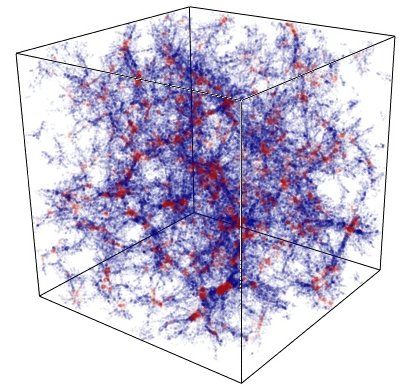
\includegraphics[width=0.9\linewidth]{LCDMstructure.jpg}
\endminipage\hfill
\minipage{0.25\textwidth}
  \centering
  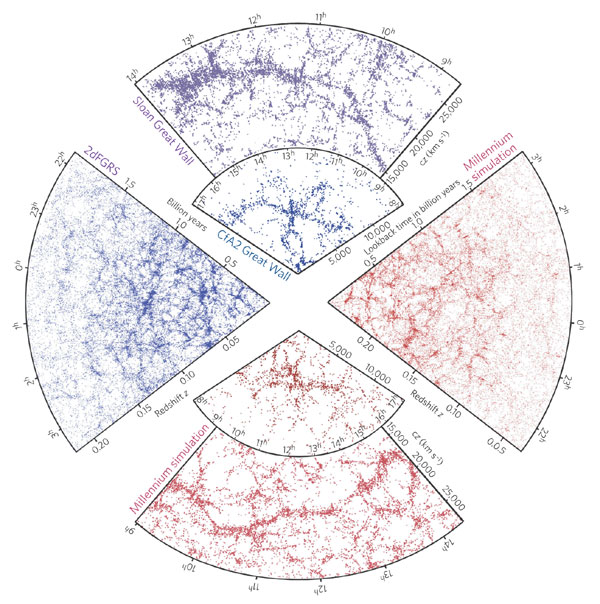
\includegraphics[width=0.9\linewidth]{nature04805-f1_2.jpg}
\endminipage\hfill
\minipage{0.50\textwidth}
  \centering
  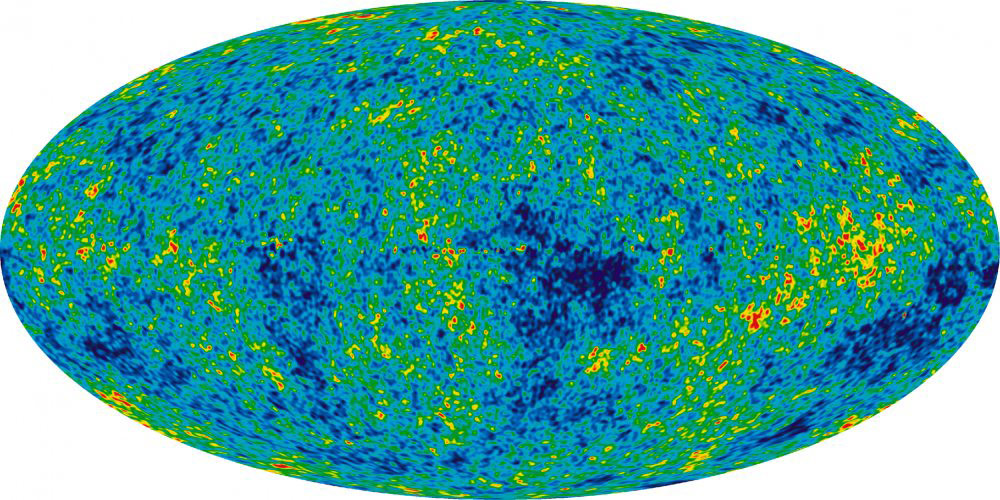
\includegraphics[width=0.8\linewidth]{simulation.jpg}
\endminipage\hfill
\caption{(Left) : A dark matter simulation cube of size 180 Mpc/h. Clusters are identified by the eigenvalues of the tidal field tensor and indicated by red colors. (Middle) : The galaxy distribution obtained from spectroscopic redshift surveys and from mock catalogues constructed from cosmological simulations. (Right) : The map of cosmic microwave background temperature fluctuations (European Space Agency Planck mission). }
\end{figure}

\section{Persistent Homology}
Persistent homology is a new approach for summarizing topological information from data. There exist different approaches to organizing point clouds into topological structure, one of the most popular being via the Rips complex. The Rips algorithm replaces the set of data points with a family of simplicial complexes, indexed by a proximity parameter. For example, a 0-simplex are points, a 1-simplex is a segment, a 2-simplex is a triangle, etc. Visually, one can think of the Rips algorithm as initially a ball at each point in the point cloud and growing the ball over a span of iterations. As the balls grow and overlap, higher dimensional complexes are formed. For example, two separate points are 0-dim complexes, but once their balls overlap, form a segment, or a 1-dim complex. As balls grow to overlap enough to fill a complex, the corresponding homological feature dies, meaning that it no longer exists. Varying the proximity parameter defines the rate of ball growing, thereby speeding up or slowing down the formation and deaths of homologies of hhigher dimensional complexes. Persistent homology then analyzes these complexes via algebraic topology, and prioritizes those complexes which persist, or span the longest lifetimes. The assumption is that the global structures which most often appear consistently are the important features. Finally, the persistent homology of the data set is encoded in the form of a parameterized version of a Betti number which is called a persistence diagram or barcode plot. These summaries provide a graphical display of the persistent homology of the data, and can potentially be used to compare against other persistent homologies.

\subsection{Uniform Circle Analysis}
A good toy model for demonstrating persistent homology is a uniform circle data set composed of $N$ independent simulations of $n$ sampled points from a uniform circle of radius $r$ and center $(0,0)$ each. One should expect the algorithm to result in $N$ different loops with similar births and deaths. The results below will show the results of persistent homology with four different $n$ values. Intuitively, one could expect a larger sample size to correlate with a more accurate topological analysis. 

\begin{figure}[!htb]
  \minipage{0.32\textwidth}
    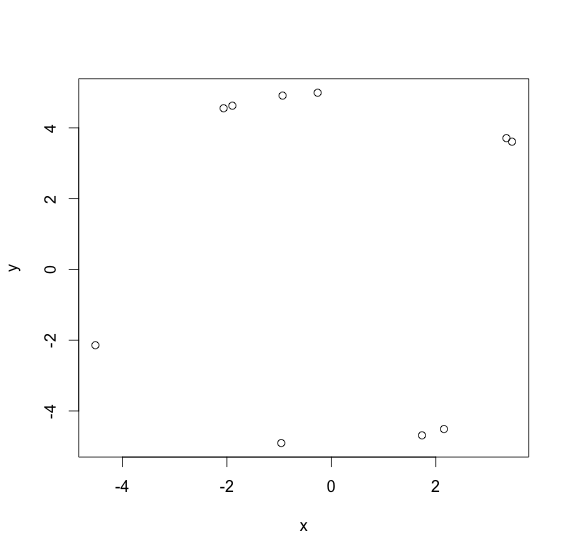
\includegraphics[width=0.85\linewidth]{circle10.png}
  \endminipage\hfill
  \minipage{0.32\textwidth}
    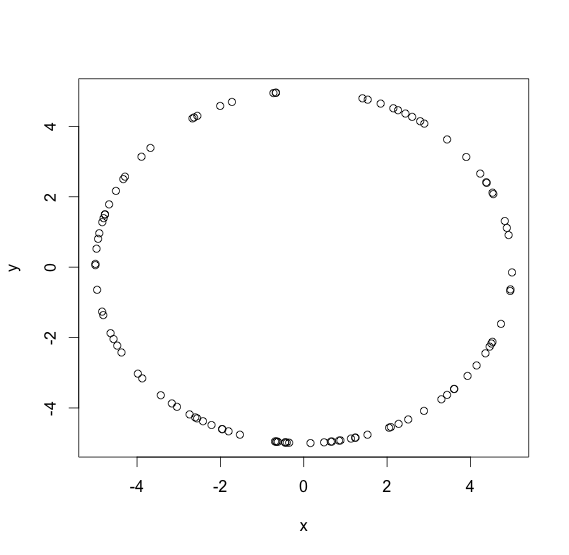
\includegraphics[width=0.85\linewidth]{circle100.png}
  \endminipage\hfill
  \minipage{0.32\textwidth}
    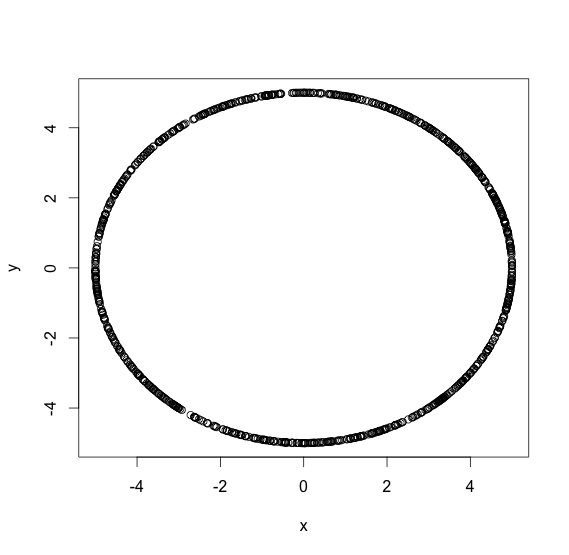
\includegraphics[width=0.85\linewidth]{circle1000.png}
  \endminipage\hfill
  \caption{Generated circles of different sample sizes. From left to right, $n$ = 10, 100, 1000. With a larger sample size, a more distinct circle is visually observable.}
\end{figure}

For each $n$ = 5, 10, 100, 250, a Rips diagram was is shown. For each of the $N$ simulations, all $N$ Rips diagrams were overlayed on top of one another. Doing so should shed light on groups of 0-dimensional, and 1-dimensional homologies like loops over repeatable simulations. 

For all Rips calculations, maxdimension is set to 1, and maxscale is set to 5. We are only looking for loops, and limit filtration to 5. Circles are centered at the origin, with a radius of 2, and 10 simulations are conducted. 

\begin{figure}[!htb]
\minipage{0.50\textwidth}
  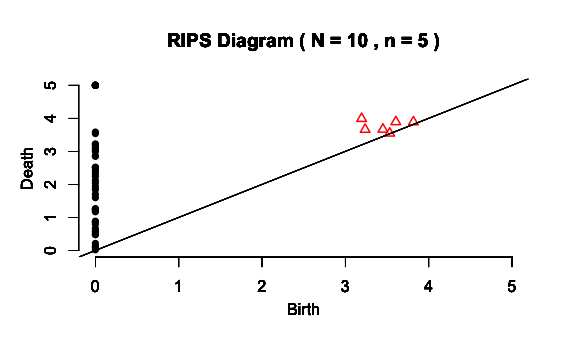
\includegraphics[width=0.8\linewidth]{RIPS_5n.png}
\endminipage\hfill
\minipage{0.50\textwidth}
  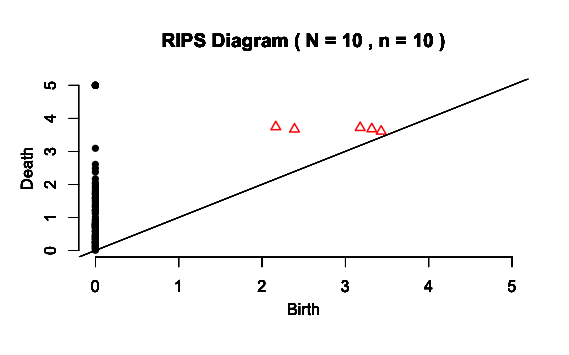
\includegraphics[width=0.8\linewidth]{RIPS_10n.png}
\endminipage\hfill
\minipage{0.50\textwidth}
  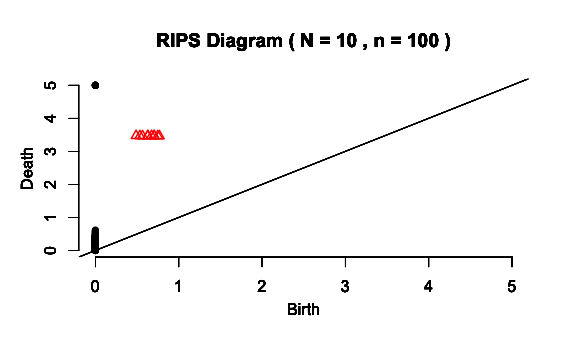
\includegraphics[width=0.8\linewidth]{RIPS_n100.png}
\endminipage\hfill
\minipage{0.50\textwidth}
  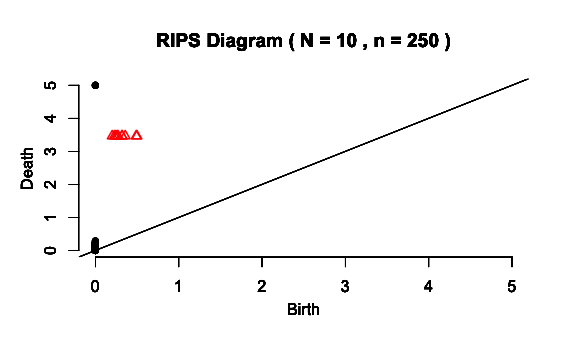
\includegraphics[width=0.8\linewidth]{RIPS_n250.png}
\endminipage\hfill
\caption{Overlapping persistence diagrams over $N$ independent simulations and varied sample sizes $n$. Generated using the TDA library in R.}
\end{figure}

Two immediately recognizable patterns are that (1) the greater the sample size (larger $n$), the earlier the detection (and formation) of higher dimensional simplicial complexes. For example, when $n = 250$, the circular loop is detected as early as 0.1 units after birth, while when $n = 5$, the loop is detection after 3.5 units..., and (2), as $n$ grows larger, the spread of deaths at time 0 is more concentrated. Compare the black points in figure 3 when $n = 5$ to when $n = 250$. Intuitively, because there are more points, more points lie on the circle's perimeter. When the balls begin to grow, the amount of growth needed to form all the overlaps to find the circle is small. Thus, the loop is found immediately. When there are very few points, the balls need much longer to grow to overlap. Therefore, given any 3 random points, there will be a loop found, even if there isn't actual structure to those three points. But most likely, that structure would not persist over time. The second observation is also explainable by the sample size. With more points, fewer initial 0-dimensional complexes appear (black points), because points start out close enough to form longer segments. When $n$ is small, the points are individual complexes, leading to increased deaths.

\section{Research Goals}
The goal of the research is to develop methods, possibly based on persistent homology, to compare probable realizations of the Universe under different sets of assumptions. Being able to appropriately analyze structure provides a standardized approach to quantitatively judge the similarities between pairs of universes. Doing so could lead to better approximations of the true initial conditions of the Universe and its development through time, along with how certain assumptions affect the topological structure.

Secondly, the ability to quantify structure may shed light on different properties and theories of dark matter. In theory, dark matter is divisible into warm and cold counterparts. Presuming that dark matter is a particle, warm dark matter particles are thought to move at ultrarelativistic speeds. Conversely, cold dark matter particles move slowly. Due to its slow velocity, cold dark matter is thought to have higher probabilities of smaller objects collapsing and merging into larger hierarchical objects. Provided that, many physicists often attribute the transformation of the initial Universe from a smooth initial state to a web-like distribution of galaxies and clusters to cold dark matter ($\lambda$CDM theory). A second research goal would be to analyze the structure of warm and cold dark matter simulations and draw conclusions on their differing physical and spatial properties. 

\begin{figure}[!htb]
	\centering
    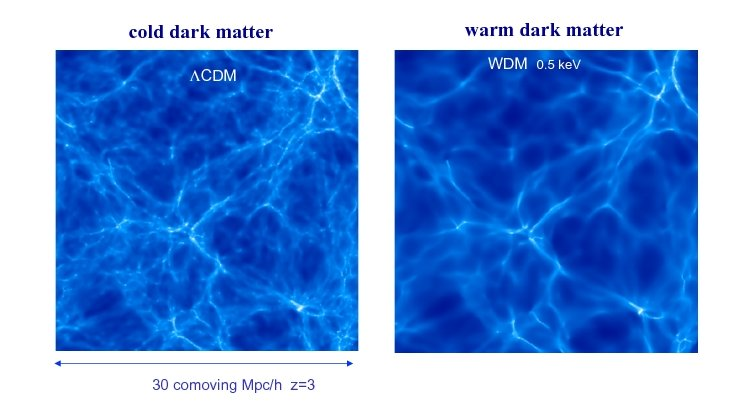
\includegraphics[width=0.5\linewidth]{simulations.jpg}
    \caption{A visual comparison between simulations of cold and warm hard matter. The streaming motions of warm dark matter suppress structure formation on small scales (Kavli Institute for Cosmology).}
\end{figure}

All research material will be hosted in a public Github repository and all computational code will be written in R and Python. 

\end{document}


